\documentclass[main.tex]{subfiles}
\begin{document}

\section{ Лекция 4 }

12 февраля

\subsection{Элементарные звенья. Продолжение}

Напомним, простейшие (элементарные) звенья -- те, передаточная функция которых имеет порядок не выше 2.

\begin{enumerate}[noitemsep]
    \setcounter{enumi}{3} % start from 4
    \item Инерционное звено

    $$ H(p) = \frac{1}{Tp + 1} \text{ -- передаточная функция } $$

    $ T $ -- \emph{постоянная времени}, параметр инерционного звена.
    Какова размерность $T$?
    Размерность $t$ -- секунды $\Rightarrow$ размерность $p$ в преобразовании Лапласа -- 1/сек, т. к. экспоненту можно брать только от безразмерной величины.

    Весовая функция: по теореме затухания

    $ h(t) = L^{-1}\{H(p)\} L^{-1}\{\frac{1}{T} \frac{1}{p + \frac{1}{T}}\} = ... = \frac{1}{T}e^{-\frac{t}{T}} $

    \textbf{Мини-задача.} Найти реакцию инерционного звена на функцию Хевисайда:
    $$ \xrightarrow{u(t)} \boxed{\frac{1}{Tp+1}} \xrightarrow{y(t)=?} $$

    $$ u(t) = 1[t], y(0) = 0 $$

    \textbf{Решение:} удобно записать в интегральной форме:

    $$ y(t) = \int_0^t h(\tau) u(t-\tau) d\tau \overset{u = 1}= 1 - e^{-\frac{t}{T}} $$

    % TODO после этой строки не проверял, хорошо ли написано

    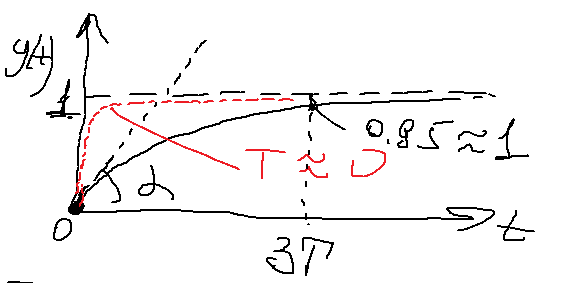
\includegraphics[width=.6\linewidth]{lec4/01_inert}

    \item Консервативное звено (сохраняет энергию)

    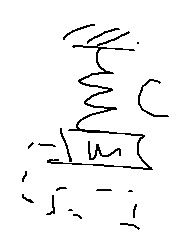
\includegraphics[width=.2\linewidth]{lec4/02_conserv_schema}

    $$ H(p) = \frac{1}{T^2p^2 + 1} $$
    Найдём весовую функцию:
    $$ h(t) = \mathcal{L}^{-1}\{\frac{1}{T} \frac{\frac{1}{T}}{p^2 + \frac{1}{T^2}}\} = \frac{1}{T} \sin(\frac{t}{T}) $$
    Обозначим $ \omega = \frac{1}{T} $
    $$ y = \frac{1}{T} \int_0^t \sin \frac{\tau}{T} \cdot 1 d \tau $$

    Незатухающие колебания

    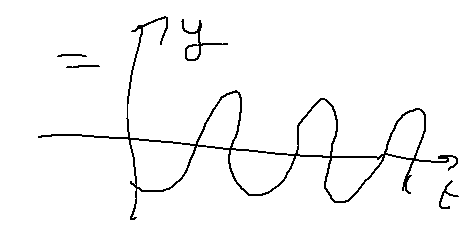
\includegraphics[width=.4\linewidth]{lec4/03_conserv_figure}

    \item Колебательное звено: обобщение консервативного ($\xi = 0$), при $\xi=1$ -- два последовательно соединённых % TODO каких?

    $$ H(p) = \frac{1}{T^2p^2 + 2 T \xi p + 1}, 0 \le \xi \le 1 $$
    \begin{align*}
        h(t) & = \mathcal{L}^{-1}\{H(p)\} = \mathcal{L}^{-1} \left\{ \frac{1}{T^2} \frac{1}{p^2 + \frac{2 \xi}{T} p + \frac{1}{T^2} + \frac{\xi^2}{T^2} - \frac{\xi^2}{T^2}} \right\} = \\
        & = \mathcal{L}^{-1} \left\{ \frac{1}{T^2 \Omega} \cdot \frac{1 \cdot \Omega}{ (p + \frac{\xi}{T})^2 + \frac{1 - \xi^2}{T^2} } \right\} \overset{ \frac{\xi}{T} = \alpha, \frac{1 - \xi^2}{T^2} = \Omega } = \frac{1}{T^2 \Omega} e^{ - \frac{\xi}{T} t} \sin \Omega t
    \end{align*}

    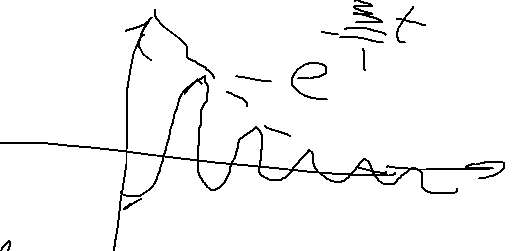
\includegraphics[width=.4\linewidth]{lec4/04_oscill}

    \begin{enumerate}[noitemsep]
        \item Звено второго порядка
        \item Корни характеристического уравнения мнимые:
        $$ p_{1,2} = - \frac{\xi}{T} \pm \Omega $$

        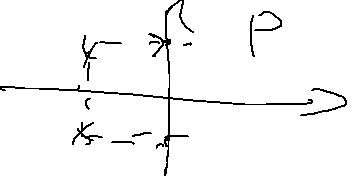
\includegraphics[width=.3\linewidth]{lec4/05_xy_roots}

    \end{enumerate}

    \item Звено чистого запаздывания

    Предположим, что система так реагирует на вход, что выход $ y(t) = u(t-\tau) $
    Схема чистого запаздывания работает во всех гаджетах.

    $$ \xrightarrow{u(t)} \boxed{H} \xrightarrow{y(t)=u(t-\tau)} $$

    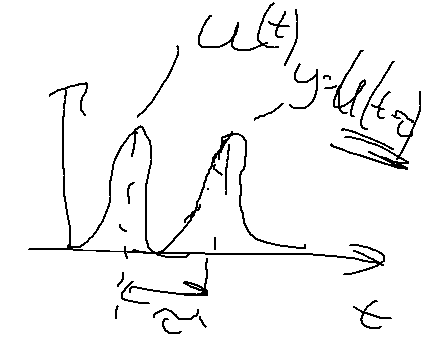
\includegraphics[width=.3\linewidth]{lec4/06_lag}

    $$ \bar y(p) = \int_{0}^{\infty} y(t)e^{-pt}dt = \int_{0}^{\infty} e^{-pt}u(t-\tau) dt \overset{t_1=t-\tau}= \int_{-\tau}^{\infty}e^{-pt_1}u(t_1)dt_1 = \bar u(p)  $$
    отсюда
    $$ \boxed{H(p)=e^{-p\tau}} $$

    Как работать с экспонентой, если мы хотим представлять в виде $ H(p) = \frac{\beta(p)}{\alpha(p)} $?

    $$ e^{-p\tau} = \frac{e^{-\frac{p\tau}{2}}}{e^{\frac{p\tau}{2}}} \approx \frac{1 - \frac{p\tau}{2} + \frac{p^2\tau^2}{8}}{1 + \frac{p\tau}{2} + \frac{p^2\tau^2}{8}} + O(\tau^2) $$ % TODO самостоятельно: вывести, поделив дробь на дробь, что остаток O(\tau^2)

    Альтернатива -- разложение Паде для числителя и знаменателя:

    $$ f(x) = \sum c_ix^i = \frac{\sum a_i x^i}{\sum b_j x^j} $$

    Доказано, что разложение Паде имеет квадратичную точность по сравнению с разложением в ряд Тейлора при одинаковом числе слагаемых.\\

    \begin{leftbar}
        Здесь было отступление: вычисление $ \sqrt x $ на основе разложения Паде.
    \end{leftbar}
\end{enumerate}

\subsection{Структурные схемы и их преобразования}

Напомним, структурная схема -- графическое изображение математического преобразования.
Разбиваем схему до элементарных звеньев (это не всегда удаётся, потому что в схеме должен наблюдаться принцип однонаправленности действия).

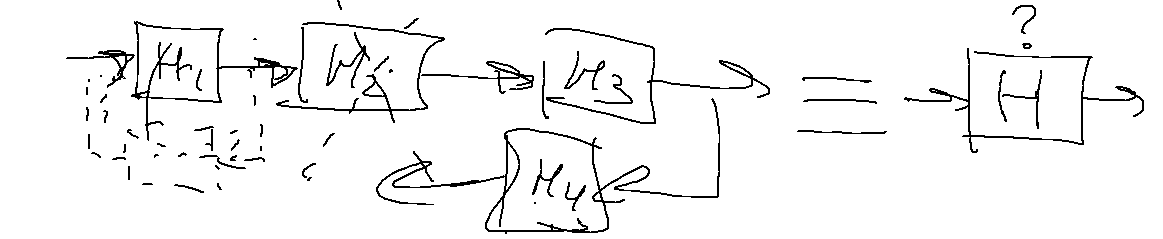
\includegraphics[width=.8\linewidth]{lec4/06_struct_scheme}

Вопрос: как объединить все звенья и написать общую функцию $ H $?

\subsubsection{Элементы структурных схем}

$$ \rightarrow \boxed{H} \rightarrow $$
\textbf{Узел:}

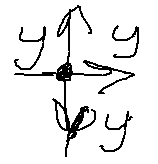
\includegraphics[width=.2\linewidth]{lec4/07_node}

Узел -- некая идеализация, считаем, что $ y $ на разветвлении идёт одинаковый в двух направлениях.

\textbf{Сумматор:}

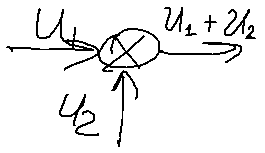
\includegraphics[width=.25\linewidth]{lec4/08_summ}

Есть сумматор с функцией вычитания (\textbf{<<вычитатор>>}):

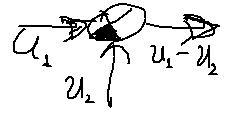
\includegraphics[width=.3\linewidth]{lec4/09_subtractor}

\subsubsection{Преобразования структурных схем}

\begin{enumerate}[noitemsep]
    \item Последовательное соединение:
    $$ \xrightarrow{u}\boxed{H_1}\xrightarrow{y_1}\boxed{H_2}\xrightarrow{y_2} $$

    $$ \boxed{H = \prod_i H_i } $$
    \item Параллельное соединение

    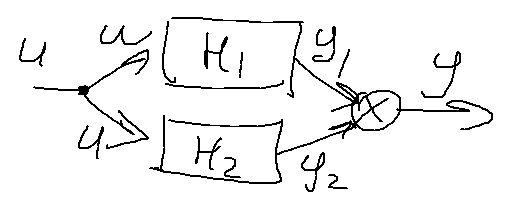
\includegraphics[width=.5\linewidth]{lec4/10_parallel}

    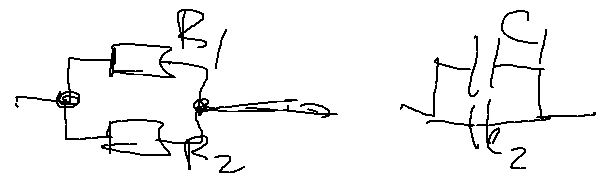
\includegraphics[width=.5\linewidth]{lec4/11_parallel_examples}

    \item Звено с обратной связью (= звено, охваченное обратной связью)

    По умолчанию обратная связь будет отрицательная.

    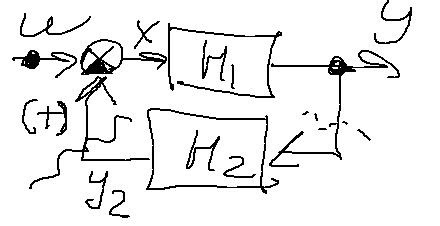
\includegraphics[width=.5\linewidth]{lec4/12_backref}

    $$ \begin{cases}
        y = H_1x \\
        x = u \mp H_2 y \thickspace (y_2 = H_2y)
    \end{cases} $$
    $$ y = H_1 (u \mp H_2 y) $$
    $$ y = \frac{H_1}{1 \pm H_1 H_2}u \Rightarrow H = \frac{H_1}{1 \pm H_1 H _2} $$

    Может быть проблемой: если $ H_1 H_2 \approx 1 $, $ H \to \infty $ (например, возникает резонанс в усилителе).

    \item Перестановка узлов. Перенос сумматора через звено

    Предположим, что по каким-то соображениям удобно объединить два звена.
    Но (см. рис) между звеньями стоит сумматор.

    \begin{enumerate}[noitemsep]
        \item Перенос вдоль стрелки:

        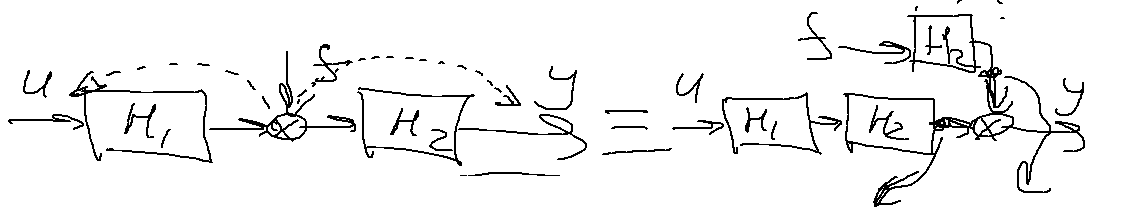
\includegraphics[width=.8\linewidth]{lec4/13_summator_transition}

        \item Перенос по стрелке:

        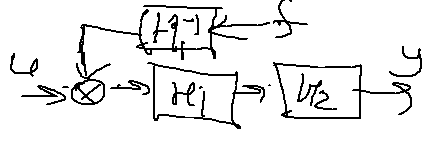
\includegraphics[width=.6\linewidth]{lec4/14_summator_transition2}

    \end{enumerate}

    \item Перенос узла по стрелке или против стрелки

    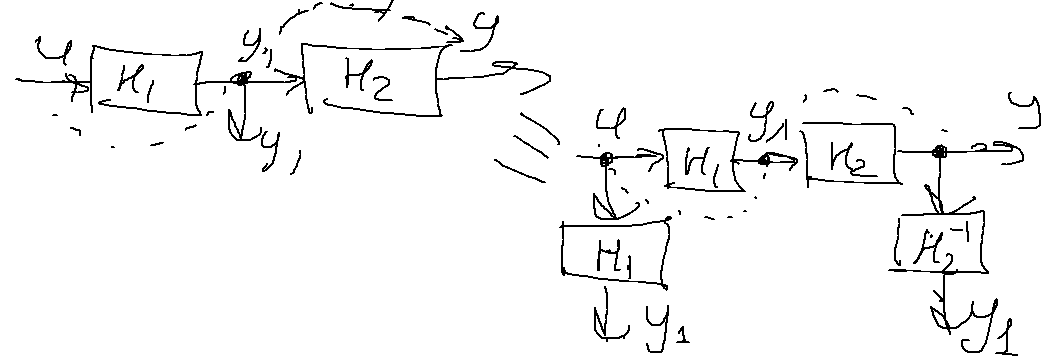
\includegraphics[width=.7\linewidth]{lec4/15_node_transition}

    Замечание: можно поставить два узла вместо одного.

    Сумматор удобно переносить по стрелке, узел -- против стрелки.

    \item Перестановка узлов и сумматоров

    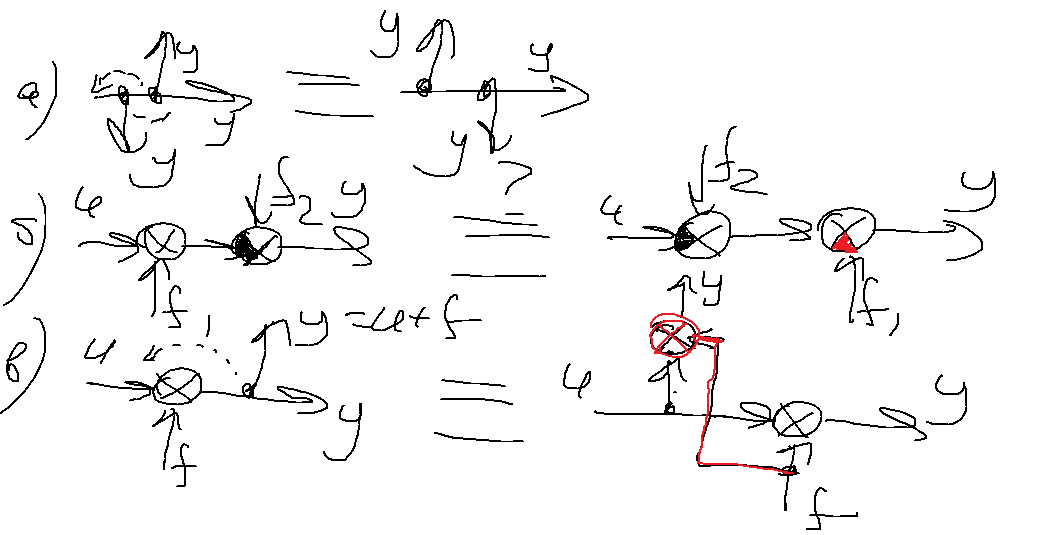
\includegraphics[width=.9\linewidth]{lec4/16_transition_examples}

     \begin{enumerate}[noitemsep]
        \item Перенос узлов
        % TODO
        \item Перенос сумматоров
        % TODO
        вычитаторы надо менять местами аккуратно.

        \item Перестановка узла и сумматора (АА: <<Мне это не нравится>>)
        % TODO
    \end{enumerate}
\end{enumerate}

\subsubsection{Вычисление передаточных функций одноконтурных систем}

\emph{Одноконтурная система}, как понятно из названия, -- та, что содержит только один замкнутый контур.

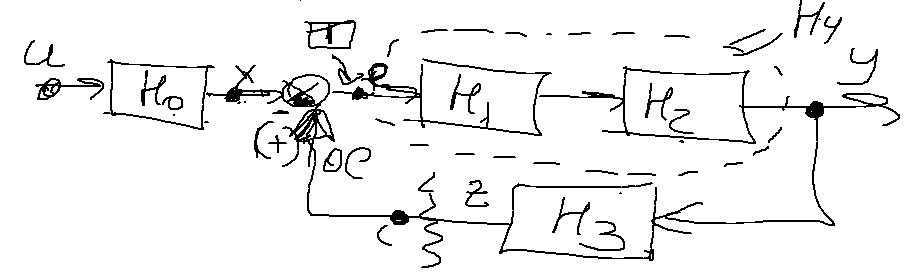
\includegraphics[width=.8\linewidth]{lec4/17_transit_func}

Пример: надо найти общую передаточную функцию $ H $.

Будем действовать последовательно.
$ H_1, H_2 $ соединены последовательно; назовём $ H_4 := H_1 H_2 $.
$ H_3, H_4 $ образуют замкнутый контур $ \Rightarrow $ их общая функция $ H_5 := \frac{H_4}{1 + H_3 H_4} $

\subsubsection{Вычисление передаточных функций в многоконтурных системах}

Если есть пересечения, нужно делать преобразования.

Можно делать преобразования геометрически или алгебраически.

Геометрически -- пример: три контура

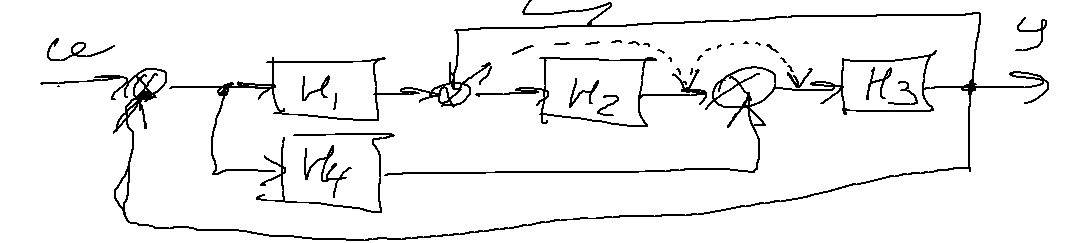
\includegraphics[width=.8\linewidth]{lec4/18_transit_multicontour}

Перенесём сумматор через звено $ H_2 $.
Поскольку нет вычитания, два сумматора после этого можно просто поменять местами.

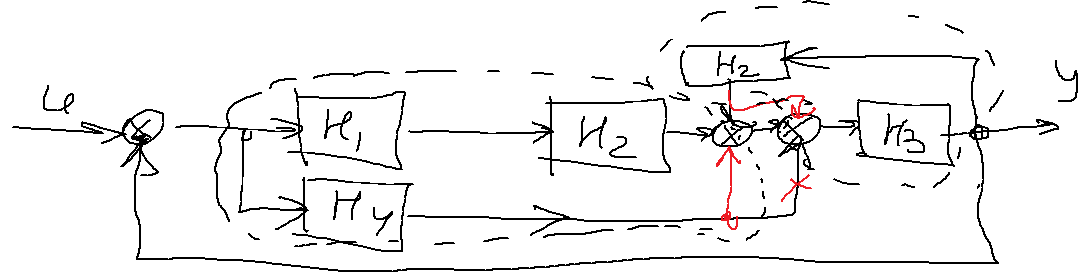
\includegraphics[width=.8\linewidth]{lec4/19_transit_multicontour2}

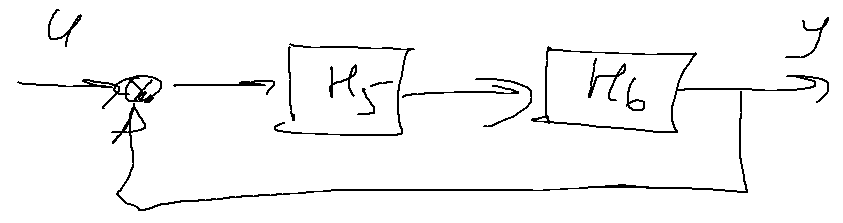
\includegraphics[width=.8\linewidth]{lec4/20_transit_multicontour3}

$$ H = H_{uy} = \frac{H_5 H_6}{1 + H_5 H_6} $$
$$ H_5 = H_1 H_2; H_6 = \frac{H_3}{1 - H_2 H_3} $$

Алгебраически:
\begin{enumerate}[noitemsep]
    \item Составляем уравнения связи для каждого звена
    \item Составляем уравнения для каждого сумматора и узла
\end{enumerate}

Если $ n $ уравнений, то переменных (значений сигнала) будет $ n + 1 $.
Исключая все переменные, кроме входной и выходной, получим зависимость: $ y = Hu $


\chapter{Устойчивость}

\subsection{Лекция 4 часть 2. Устойчивость. Введение}

Потеря устойчивости -- это аварии, катастрофы, жертвы...

Важно идентифицировать нарушения устойчивости.
Это помогает делать неустойчивую систему устойчивой.

Рассмотрим произвольную систему с управляющим воздействием $u$, возмущающим $W$ и выходом $y$.

$$ \xrightarrow{u} \overset{\downarrow W}{\boxed{\text{ОУ}}} \xrightarrow{y} $$

\emph{Устойчивая система} -- та, выход которой мало меняется при малых изменениях воздействий и параметров.

\textbf{Примеры:}
\begin{enumerate}
    \item Маятник грузиком вверх: устойчивый, грузом вниз -- неустойчивый
    \item Пассажирские самолёты: хвостовое оперение $ \Rightarrow $ устойчивая схема.
    Истребитель, построенный по схеме <<Утка>>: неустойчивый (планировать не может), зато маневренный.
    \item Хвостовое оперение ракеты или стрелы: служит для устойчивости.
    \item Прямолинейная езда при езде на велосипеде или автомобиле является устойчивой, потому что при повороте руля центр масс транспортного средства приподнимается (так сконструировано).
\end{enumerate}

\subsubsection{Формальный пример неустойчивого объекта}

$$ \xrightarrow{u} \overset{\downarrow W}{\otimes} \rightarrow \boxed{\frac{1}{D-1}} \xrightarrow{y} $$

\begin{align*}
    & y = \frac{1}{D-1}(u+w) \\
    & \dot y - y = u + w \\
\end{align*}

\begin{enumerate}
    \item ] н. у. $y(0)=0, W=W_0=const$.
    $u=? : y(t)=0 \forall t$

    Решим задачу так: $ ] u = u_{\text{пр}} = - W_0 $ (программное управление).

    Тогда $ \dot y - y = 0 \Rightarrow y(t) \equiv 0 $.

    \item ] всё то же, но $ W = W_0 + \Delta W = const $.

    Программное управление $ u = u_{\text{ прогр }} = - W_0 $ $ \Rightarrow $ $ \dot y - y = \Delta W $.

    Решение такого ДУ
    \[ y(t) = c e^t + y_{\text{частн}} = ce^t - \Delta W  \]
    Из начальных условий $ C = \Delta W  \Rightarrow $ $ y(t) = \Delta W (e^t - 1) $.

    Решение стремится к бесконечности при $t \to \infty $!

    Значит, система неустойчива.
    Когда система неустойчива, программное управление плохо.

    \item Что, если начальные условия не совсем нулевые?
    \[ ] W = W_0 = const, \text{н. у. } y(0) = \varepsilon \ne 0 \]
    \[ y(t) = ce^t + \varepsilon \]

    Тоже решение стремится к бесконечности.
\end{enumerate}

\subsubsection{Строгое определние: устойчивость по Ляпунову (1892 г)}

Ляпунов дал определение устойчивости для произвольной, в том числе нелинейной, системы.
Три определения (и перед ними <<нулевое>>):

\begin{enumerate}
    \item[0.] $ ] X(0) = X_0 \to  X^*(t) $ -- решение при невозмущённых начальных условиях.

    Когда вносим возмущение в начальные условия, поведение системы меняется:

    \[ X(0) = X_0 + \Delta X_0 \to X(t) = X^*(t) + \Delta X(t) \]

    \begin{enumerate}[noitemsep]
        \item Если малому отклонению в начальный момент соответствует малое отклонение в следующие моменты времени $ \Delta X(t) $, система называется \emph{ устойчивой } (по Ляпунову).

        \item Если малому отклонению в н. у. соответствует нарастающее отклонение $ \Delta X)(t) \to \infty $, система называется \emph{ неустойчивой }.

        \item Если малому отклонению в н. у. соответствует исчезающе малое отклонение $ \Delta X \xrightarrow[t \to \infty]{} 0 $, систему называют \emph{асимптотически устойчивой}.
    \end{enumerate}

    \item Определение на языке $\varepsilon, \delta$:

    $ \forall \varepsilon > 0 \exists \delta > 0 : ||\Delta X_0|| \le 0 \Rightarrow ||Delta X(t)|| \le \varepsilon $

    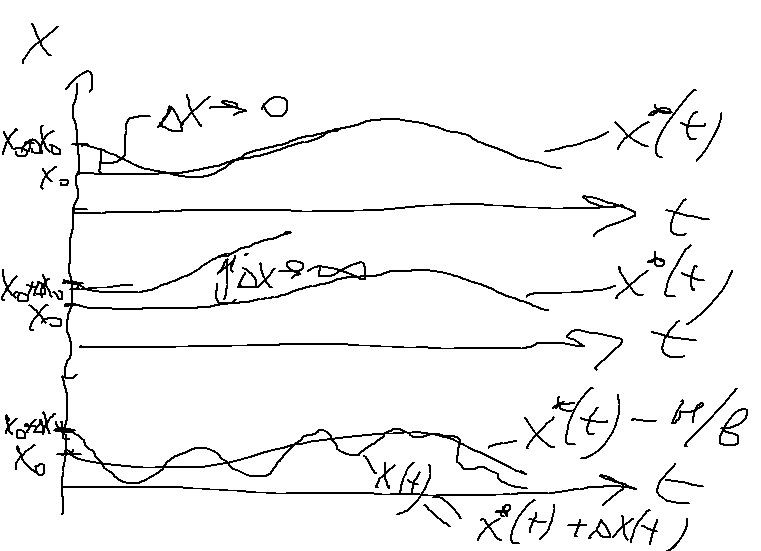
\includegraphics[width=.8\linewidth]{lec4/21_stability}

    Нижняя картинка: устойчивое поведение, средняя: неустойчивая, верхняя -- асимптотически устойчивое.
\end{enumerate}

В теории управления, как правило, стремятся построить асимптотически устойчивую систему.

\subsubsection{Необходимые и достаточные условия асимптотической устойчивости для ЛСАУ}

Напомним, ЛСАУ -- линейная система автоматического управления.

$$ \xrightarrow{u} \boxed{\frac{\beta(D)}{\alpha(D)}} \xrightarrow{y} \Leftrightarrow \alpha(D)y=\beta(D)u $$

Пусть
\begin{itemize}[noitemsep]
    \item $y^*(t)$ -- выход при невозмущённом входе, соотв. $y_0, ...$;
    \item $y(t) $ -- возмущённое решение, соответствующее $y_0 + \Delta y_0, ...$
\end{itemize}

Введём $ \Delta y(t) := y(t) - y^*(t) $.

\[ \alpha y^* = \beta u \]
\[ \boxed{ \alpha(D) \Delta y = 0 } \]
На устойчивость влияют только внутренние свойства системы -- коэффициенты характеристического многочлена $ \alpha $.

Если $ \Delta y = e^{\lambda t} $, то $ \Delta \dot y = \lambda e^{\lambda t} $ и т. д.

Приходим к уравнению:
\[ \alpha_n \lambda^{n} e^{\lambda t} + ... + \alpha_1 \lambda e^{\lambda t} + \alpha_0 e^{\lambda t} = 0 \]
Сокращаем экспоненту:
\[ \boxed{ \alpha(\lambda) = 0 } \]
это -- \emph{ характеристическое уравнение }.

Обозначим $ \{  \lambda_i \} $ -- корни.

$ \Delta y(t) = \sum_i C_i e^{\lambda_i t} $ при $ \lambda_i $ различных.

Если есть кратные корни, появятся т. н. <<вековые>> слагаемые.

$\lambda_1 = \lambda_2 (= ...) \Rightarrow \Delta y = C_1 e^{\lambda_1 t} + C_1 t e^{\lambda_1 t} (+ ...) $

Иной подход к проблеме одинаковых корней -- инженерный: можно считать, что $ \lambda_1 = \lambda_2 + \varepsilon $ (отличаются на исчезающе малую добавку; формально различные).

\begin{enumerate}[noitemsep]
    \item $ ] \lambda_i $ вещественные, $ \Delta y = \sum C_i e^{\lambda_i t} $ $ \Leftrightarrow $ условие устойчивости -- $ \boxed{ \lambda_i < 0 } $
    \item Если $ \lambda_i $ комплексно сопряжённые:
    \[ ] \begin{cases}
        \lambda_1 = a + jb \\
        \lambda_2 = a - jb
    \end{cases} \]
    \begin{align*}
        \Delta y & = C_1 e^{\lambda_1 t} + C_2 e^{\lambda_2 t} + ... = \\
        & = e^{at} \left[ C_1 (\cos bt + j \sin bt) + C_2 (\cos bt - j \sin bt) \right] = \\
        & = e^{at}[D_1 \cos bt + D_2 \sin bt] = \boxed{ e^{at} A \cos(bt + \phi) }
    \end{align*}

    Т. о. условие устойчивости -- $ a < 0 $.
\end{enumerate}

В общем случае: корни должны лежать в левой полуплоскости комплексной плоскости.

\end{document}
